% This is LLNCS.DEM the demonstration file of
% the LaTeX macro package from Springer-Verlag
% for Lecture Notes in Computer Science,
% version 2.3 for LaTeX2e
%
\documentclass{llncs}
%
\usepackage{makeidx}  % allows for indexgeneration
\usepackage{amsmath,amssymb,url,graphicx,graphics,ifthen,epsfig,algorithm,algorithmic,multirow}


\begin{document}
%

\title{Biasing Monte-Carlo Simulations through RAVE Values}
%
\titlerunning{Rave Based Monte-Carlo}  % abbreviated title (for running head)
%                                     also used for the TOC unless
%                                     \toctitle is used
%
\author{Arpad Rimmel\inst{1} \and
	Fabien Teytaud\inst{2} \and
	Olivier Teytaud\inst{2}
}
%
\institute{
Department of Computing Science,
University of Alberta,
Canada,
rimmel@cs.ualberta.ca
\and
TAO (Inria), LRI, UMR 8623(CNRS - Univ. Paris-Sud),\\ bat 490 Univ. Paris-Sud 91405 Orsay, France}

\maketitle              % typeset the title of the contribution

\begin{abstract}
The Monte-Carlo Tree Search algorithm has been successfully applied in various domains. However, its performance heavily depends on the Monte-Carlo part. In this paper, we propose a generic way of improving the Monte-Carlo simulations by using RAVE values, which already strongly improved the tree part of the algorithm. We prove the generality and efficiency of our approach by showing improvements on two different applications: the game of Havannah and the game of Go. 
\end{abstract}
%
\section{Introduction}



Monte-Carlo Tree Search (MCTS) \cite{chaslot06a,coulom06,uct} is a recent algorithm for taking decisions in a discrete, observable, uncertain environment with finite horizon. The algorithm is particularly interesting when the number of states is huge.
In this case, classical algorithms such as Minimax and Alphabeta \cite{knuth1975analysis}, for two-player games, and Dynamic Programming \cite{adp}, for one-player games, are too time-consuming or not efficient. 
MCTS combines an exploration of the tree based on a compromise between exploration and exploitation, and an evaluation based on Monte-Carlo simulations. A classical generic improvement is the use of the RAVE values \cite{icmlmogo}. The corresponding algorithm and its improvement will be described in section \ref{MCTS}.
It achieved particularly good results in two-player games such as computer Go \cite{ieeemogo} and Havannah \cite{fabienHavannah}. Moreover, it was also successfully applied on one-player problems such as the automatic generation of libraries for linear transforms \cite{icmlrimmel}, non-linear optimization \cite{unleo}, and active learning \cite{roletecml}.


The algorithm can be improved by modifying the Monte-Carlo simulations. For example, in \cite{mogofpu}, the addition of patterns to the simulations leads to a significant improvement in the case of the game of Go. However, those patterns are domain-specific. In this paper, we propose a generic modification of the simulations based on the RAVE values that we called ``poolRave''. The principle is to play moves that are considered efficient according to the RAVE values with a higher probability than the other moves. We show significant positive results on two different applications: the game of Go and the game of Havannah.


We first present the principle of the Monte-Carlo Tree Search algorithm and of the RAVE improvement (section \ref{MCTS}). Then, we introduce the new Monte-Carlo simulations (section \ref{poolrave}). Subsequently, we present the experiments (section \ref{xp}). Finally, conclusions are given and future work is announced (section 5).


\section{Monte-Carlo Tree Search}\label{MCTS}

MCTS is based on the incremental construction of a tree representing the possible future states by using (i) a bandit formula (ii) Monte-Carlo simulations. Subsection \ref{bdts} presents bandits and subsection \ref{mct} then presents their use for planning and games, i.e., MCTS.

\subsection{Bandits}\label{bdts}

A $k$-armed bandit problem is defined by the following elements.
\begin{itemize}
        \item A finite set of arms is given; without loss of generality, the set of arms can be denoted $J=\{1,\dots,k\}$.
        \item Each arm $j\in J$ is equipped with an unknown random variable $X_j$; the expectation of $X_j$ is denoted $\mu_j$.
        \item At each time step $t\in \{1,2,\dots\}$:
	\begin{itemize}
		\item the algorithm chooses $j_t\in J$ depending on $(j_1,\dots,j_{t-1})$ and $(r_1,\dots,r_{t-1})$;
        	\item each time an arm $j$ is selected, the algorithm obtains a reward $r_t$, which is an independent realization of $X_{j_t}$.
	\end{itemize}
\end{itemize}

The goal of the problem is to minimize the so-called {\em{regret}}.
Let $T_j(n)$ be the number of times an arm has been selected during the first $n$ steps.
The {\em{regret}} after $n$ steps is defined by
$$ \mu^* n - \sum_{j=1}^{k}{\mu_j  \mathbb{E}[T_j(n)]}  \textrm{ where }  \mu^*=\max_{1 \le i \le k} \mu_i. $$

 $\mathbb{E}[T_j(n)]$ represents the esperance of $T_j(n)$.

In \cite{auer}, the authors achieve a logarithmic regret (it has been proved  in \cite{lairobbins}) that this is the best obtainable regret) independently of the $X_j$ with the following algorithm: first, try one time each arm; then, at each step, select the arm $j$ that maximizes
\begin{equation}
\bar{x_j} + \sqrt{\frac{2ln(n)}{n_j}}.
\label{ucb}
\end{equation}

$\bar{x_j}$ is the average reward for the arm $j$ (until now). $n_j$ is the number of times the arm $j$ has been selected so far. $n$ is the overall number of trials so far.
This formula consists in choosing at each step the arm that has the highest upper confidence bound (UCB). It is called the UCB formula.


\subsection{Monte-Carlo Tree Search}\label{mct}

The MCTS algorithm constructs in memory a subtree $\hat{T}$ of the global tree $T$ representing all the possible future states of the problem (the so-called extensive form of the problem).
The construction of $\hat T$ is done by the repetition (while there is some time left) of 3 successive steps: {\em{descent, evaluation, growth}}.
The algorithm is given in Alg. \ref{cmcalgo} (Left)  and illustrated in Fig. \ref{uctfig}.
\begin{figure}[htb]
\begin{center}
%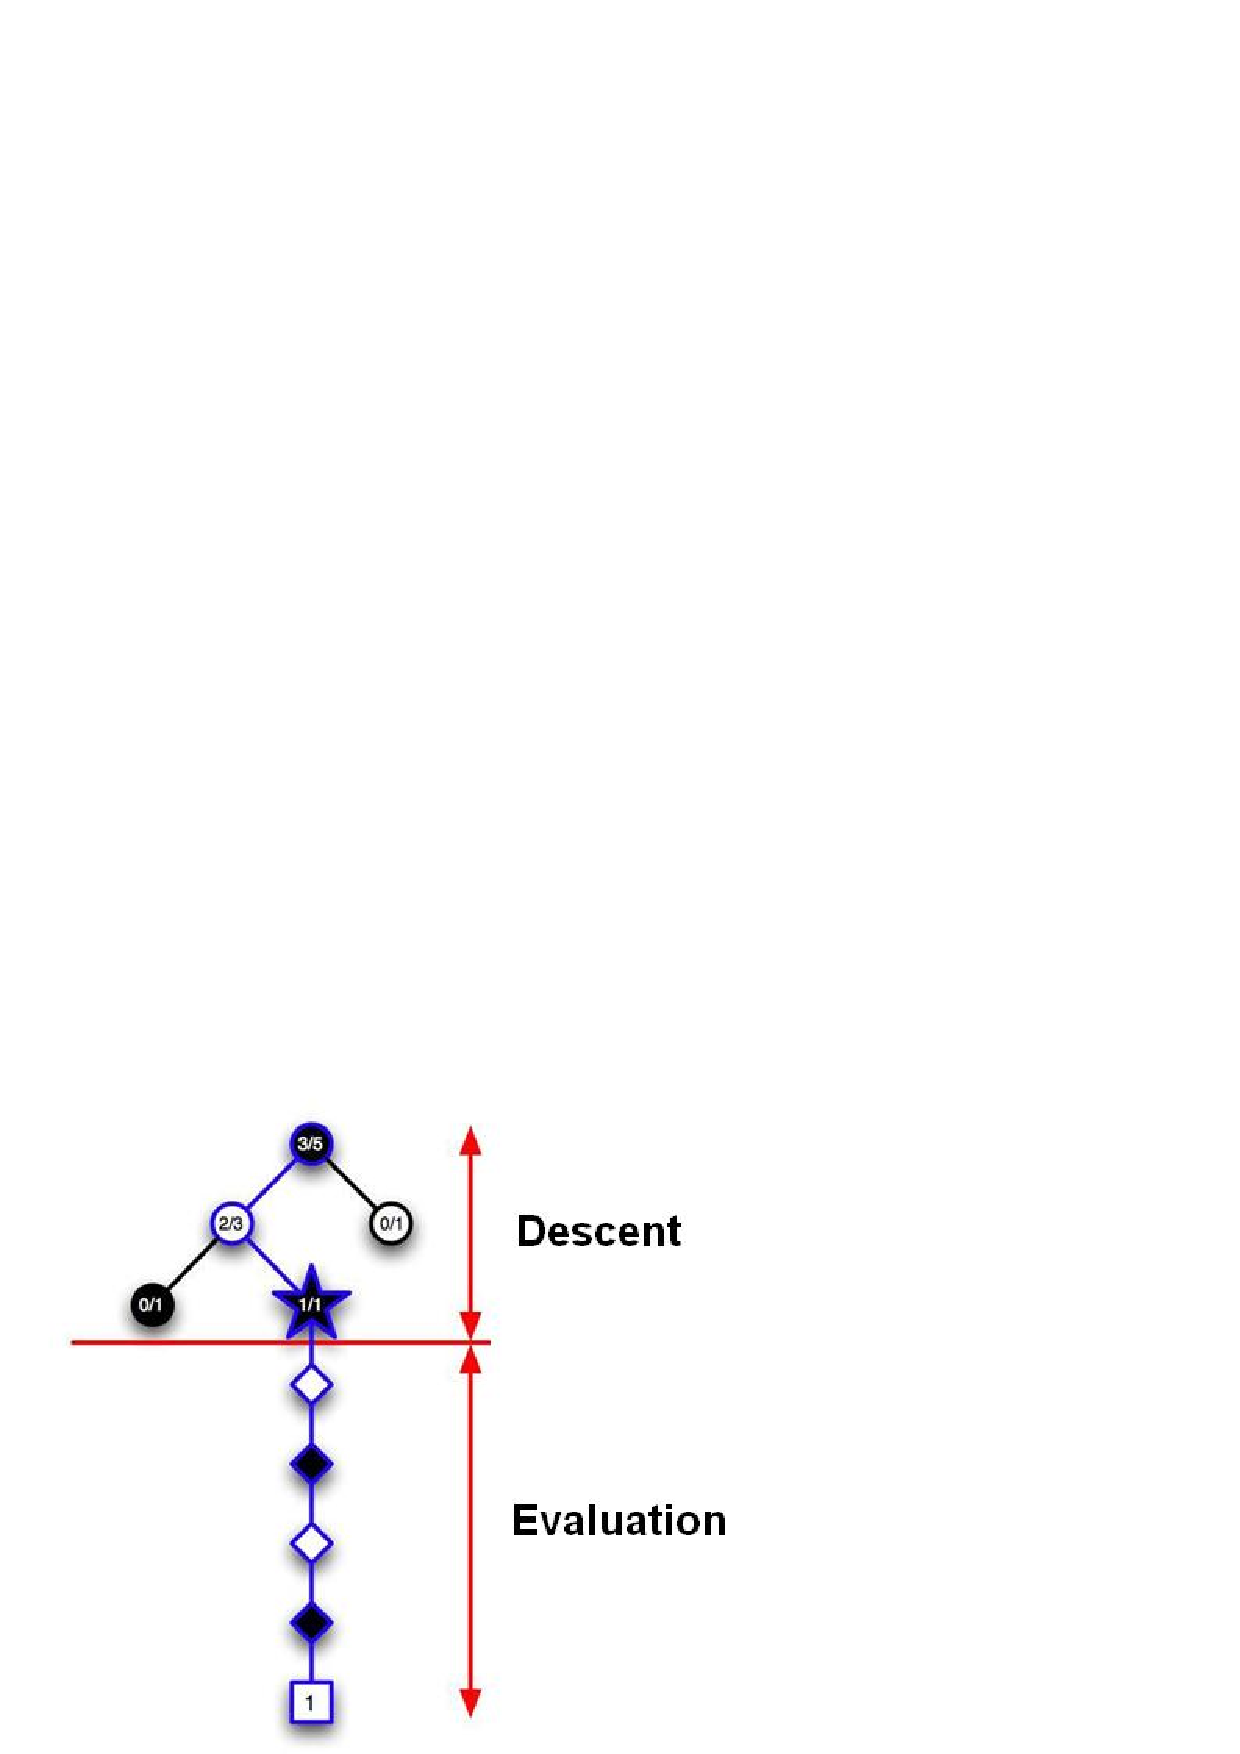
\includegraphics[width=5cm]{uctfig.jpg}
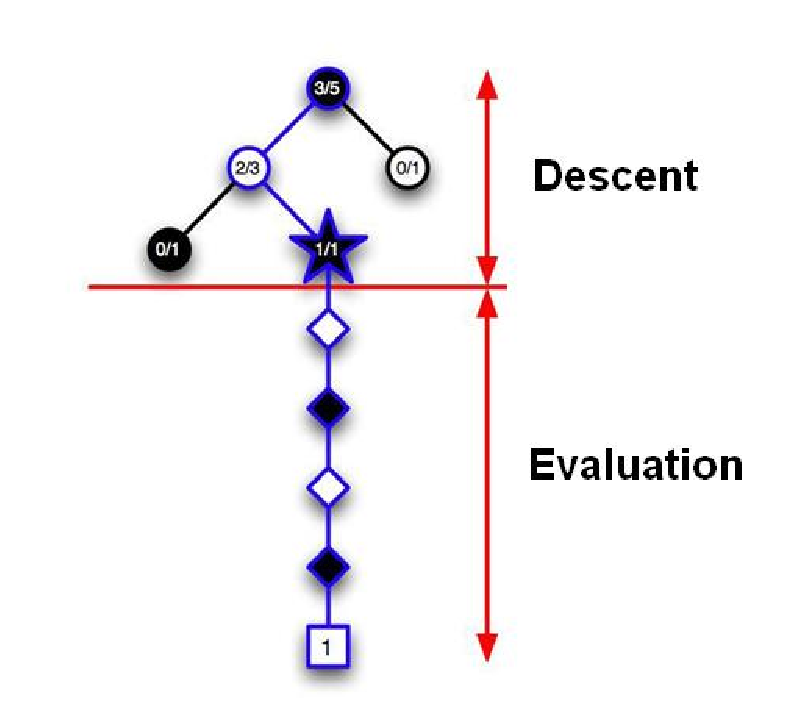
\epsfig{file=uctfig.eps,width=5cm}
\end{center}
\caption{\label{uctfig} Illustration of the Monte-Carlo Tree Search algorithm from a presentation of the article \cite{icmlmogo}}
% $\hat{T}$ is represented by the circles. A Monte-Carlo simulation is represented by the diamonds. The node added to the tree ($S$) is represented by the star and the terminal state associated to the reward is represented by the square.}
\end{figure}

{\bf{Descent.}} The descent in $\hat{T}$ is done by considering that selecting a new node is equivalent to a $k$-armed bandit problem. In each node $s$ of the tree, the following information items are stored:
\begin{itemize}
\item $n_s$: the total number of times the node $s$ has been selected;
\item $\bar{x_s}$: the average reward for the node $s$.
\end{itemize}
The formula to select a new node $s'$ is based on the UCB formula \ref{ucb}.
Let $C^s$ be the set of children of the node $s$:
$$ s' \leftarrow  \operatorname*{arg\,max}\limits_{j \in C^s}{\bar{x_j} + \sqrt{\frac{2ln(n_{s})}{n_j}}}. $$
Once a new node has been selected, we repeat the same principle until we reach a situation $S$ outside of $\hat{T}$.

{\bf{Evaluation.}}
Now that we have reached a situation $S$ outside of $\hat{T}$. There is no more information available to take a decision; as in the tree, we cannot use the bandit formula. As we are not at a leaf of $T$, we cannot directly evaluate $S$. Instead, we use a Monte-Carlo simulation to have a value for $S$. The Monte-Carlo simulation is done by selecting a new node (a child of $s$) using the heuristic function $mc(s)$ until a terminal node is reached.
$mc(s)$ returns one element of $C^s$ based on a uniform distribution (in some cases, better distributions than the uniform distribution are possible; we will consider uniformity here for Havannah, and the distribution in \cite{mogofpu} for the game of Go).  
 

{\bf{Growth.}}
In the growth step, we add the node $S$ to $\hat{T}$. In some implementations, the node $S$ is added to the node only after a finite fixed number of simulations instead of just $1$; this number is $1$ for our implementation for Havannah and $5$ in our implementation for Go.  

After adding $S$ to $\hat T$, we update the information in $S$ and in all the situations encountered during the descent with the value obtained with the Monte-Carlo evaluation (the numbers of wins and the numbers of losses are updated).

\begin{algorithm}
\begin{center}
\begin{scriptsize}
\begin{tabular}{p{0.5\linewidth}|p{0.5\linewidth}}

\begin{minipage}[p]{\linewidth}

\begin{algorithmic}
\STATE{Initialization of $\hat{T}$, $n$, $\bar{x}$}
\WHILE{there is some time left}
\STATE{$s' \leftarrow s$}
\STATE{Initialization of $game$}
\STATE{//{\it{DESCENT}}//}
\WHILE{$s'$ in $\hat{T}$ and $s'$ not terminal}
\STATE{$s' \leftarrow \operatorname*{arg\,max}\limits_{j \in C^{s'}}{[\bar{x_j} + \sqrt{\frac{2ln(n_{s'})}{n_j}}]}$}
\STATE{$game \leftarrow game + s'$}
\ENDWHILE
\STATE{$S=s'$}
\STATE{//{\it{EVALUATION}}//}
\WHILE{$s'$ is not terminal}
\STATE{$s' \leftarrow mc(s')$}
\ENDWHILE
\STATE{$r=result(s')$}
\STATE{//{\it{GROWTH}}//}
\STATE{$\hat{T} \leftarrow \hat{T} + S$}
\FOR{each $s$ in $game$}
\STATE{$n_{s} \leftarrow n_{s} + 1$}
\STATE{$ \bar{x_s} \leftarrow (\bar{x_s}* (n_{s}-1) +r ) / n_s $}
\ENDFOR
\ENDWHILE
\end{algorithmic}

       \end{minipage}
&


        \begin{minipage}[p]{\linewidth}

\begin{algorithmic}
\STATE{Initialization of $\hat{T}$, $n$, $\bar{x}$, $n^{RAVE}$, $\bar{x}^{RAVE}$}
\WHILE{there is some time left}
\STATE{$s' \leftarrow s$}
\STATE{Initialization of $game$, {\bf{$simulation$}}}
\STATE{//{\it{DESCENT}}//}
\WHILE{$s'$ in $\hat{T}$ and $s'$ not terminal}
\STATE{$s' \leftarrow \operatorname*{arg\,max}\limits_{j \in C^{s'}}{[\bar{x_j} + {\bf{ \alpha \bar{x}_{s',j}^{RAVE}}} +\sqrt{\frac{2ln(n_{s'})}{n_j}}]}$}
\STATE{$game \leftarrow game + s'$}
\ENDWHILE
\STATE{$S=s'$}
\STATE{//{\it{EVALUATION}}//}
\STATE{//beginning of the poolRave modification //}
\STATE{$s''\leftarrow $ last visited node in the tree with at least $50$ simulations}
\WHILE{$s'$ is not terminal}
\IF{Random $<p$}
\STATE{$s' \leftarrow $one of the $k$ moves with best RAVE value in $s''$}
\STATE{\hfill /* this move is randomly and uniformly selected */}
\ELSE
\STATE{$s' \leftarrow mc(s')$}
\ENDIF
\STATE{$simulation \leftarrow simulation + s'$}
\ENDWHILE
\STATE{//end of the poolRave modification //}
\STATE{//without poolRave, just $s'\leftarrow mc(s')$//}
\STATE{$r=result(s')$}
\STATE{//{\it{GROWTH}}//}
\STATE{$\hat{T} \leftarrow \hat{T} + S$}
\FOR{each $s$ in $game$}
\STATE{$n_{s} \leftarrow n_{s} + 1$}
\STATE{$ \bar{x_s} \leftarrow (\bar{x_s}* (n_{s}-1) +r ) / n_s $}
\FOR{each $s'$ in $simulation$}
\STATE{$ {\bf{n_{s,s'}^{RAVE} \leftarrow n_{s,s'}^{RAVE} + 1}}$}
\STATE{$ {\bf{\bar{x}_{s,s'}^{RAVE} \leftarrow ({\bar{x}_{s,s'}^{RAVE}}*({n_{s,s'}^{RAVE}}-1) +r )/{n_{s,s'}^{RAVE}}}} $}
\ENDFOR
\ENDFOR
\ENDWHILE
\end{algorithmic}

       \end{minipage}

\end{tabular}


\caption{\label{cmcalgo}{\bf{Left.}} MCTS($s$) {\bf{Right.}} RMCTS($s$), including the poolRave modification.//$s$ a situation.}

\end{scriptsize}
\end{center}
\end{algorithm}


\subsection{Rapid Action Value Estimates}

This section is only here for introducing notations and recalling the principle of rapid action value estimates; people who have never seen these notions are referred to \cite{icmlmogo} for more information.
One generic and efficient improvement of the Monte-Carlo Tree Search algorithm is the RAVE values introduced in \cite{bruegmann,icmlmogo}.
In this subsection we note $f\to s$ the move which leads from a node $f$ to a node $s$ ($f$ is the father and $s$ the child node corresponding to move $m=f\to s$).
The principle is to store, for each node $s$ with father $f$, 
\begin{itemize}
\item the number of wins (won simulations crossing $s$ - this is exactly the number of won simulations playing the move $m$ in $f$);
\item the number of losses (lost simulations playing $m$ in $f$);
\item the number of AMAF\footnote{AMAF$=$All Moves As First.} wins, i.e., the number of won simulations such that $f$ has been crossed and $m$ has been played after situation $f$ by the player to play in $f$ (but not necessarily in $f$!). In MCTS, this number is termed RAVE wins (Rapid Action Value Estimates);
\item and the number of AMAF losses (defined similarly to AMAF wins).
\end{itemize} 
%%%%%%and for games starting from $s$ and in wich a specific move $s'$ has been played. We don't consider when the move $s'$ has been played during the game. this value is noted $\bar{x}_{s,s'}^{RAVE}$.
The percentage of wins established with RAVE values instead of standard wins and losses is noted $\bar{x}_{f,s}^{RAVE}$.
The total number of games starting from $f$ and in which $f\to s$ has been played is noted $n_{f,s}^{RAVE}$.

From the definition, we see that RAVE values are biased; a move might be considered as good (according to $\bar{x}_{f,s}$) just because it is good later in the game; equivalently, it could be considered as bad just because it is bad later in the game, whereas in $f$ it might be a very good move.

Nonetheless, RAVE values are very efficient in guiding the search: each Monte-Carlo simulation updates many RAVE values per crossed node, whereas it updates only one standard win/loss value. Thanks to these bigger statistics, RAVE values are said to be more biased but to have less variance.

Those RAVE values are used to modify the bandit formula \ref{ucb} used in the {\it{descent}} part of the algorithm. The new formula to chose a new node $s'$ from the node $s$ is given below; let $C^s$ be the set of children of the node $s$.

$$ s' \leftarrow  \operatorname*{arg\,max}\limits_{j \in C^s}{[\bar{x_j} + {\bf{ \alpha \bar{x}_{s,j}^{RAVE}}} + \sqrt{\frac{2\ln(n_{s})}{n_j}}]} $$


$\alpha$ is a parameter that tends to $0$ with the number of simulations.
When the number of simulations is small, the RAVE term has a larger weight in order to benefit from the low variance.
When the number of simulations gets high, the RAVE term becomes small in order to avoid the bias. Please note that the right hand term $+\sqrt{\frac{2\ln(n_s)}{n_j}}$ exists in the particular case UCT; in many applications, the constant $2$ is replaced by a much smaller constant or even $0$; see \cite{ieeemogo} for more on this.

The modified MCTS algorithm with RAVE values is given in Alg. \ref{cmcalgo} (Right); it includes also the poolRave modification described below. The modifications corresponding to the addition of the RAVE values are put in bold and the poolRave modification is delimited by text.

\section{PoolRave}\label{poolrave}

The contribution of this paper is to propose a generic way to improve the Monte-Carlo simulations. A main weakness of MCTS is that choosing the right Monte-Carlo formula ($mc(.)$ in Alg. \ref{cmcalgo}) is very difficult; the sophisticated version proposed in \cite{mogofpu} made a big difference with existing functions, but required a lot of human expertise and work. We aim at reducing the need for such expertise.
The modification is as follows:
before using $mc(s)$, and with a fixed probability $p$, try to choose one of the $k$ best moves according to RAVE values. The RAVE values are those of the last node with at least $50$ simulations.
We will demonstrate the generality of this approach by proposing two different successful applications: the classical application to the game of Go, and the interesting case of Havannah in which far less expertise is known.


\section{Experiments}\label{xp}

We will consider (i) Havannah (subsection \ref{hav}) and then the game of Go (subsection \ref{go}).

\subsection{Havannah}\label{hav}

We will briefly present the rules and then our experimental results.

The game of Havannah is a two-player game created by Christian Freeling. The game is played on a hexagonal board with hexagonal locations. It can be considered as a connection game, like the game of Hex or Twixt. 
The rules are straightforward. White starts, and after that each player plays alternatively. To win a game a player has to realize one of these three shapes.
\begin{itemize}
\item A ring, which is a loop around one or more cells (empty or not, occupied by black or white stones).
\item A bridge, which is a continuous string of stones that connects one of the six corners to another one.
\item A fork, which is a continuous string of stones that connects three of the six sides of the board (corner locations are not belonging to the edges).
\end{itemize}

An example of these three winning positions is given in Fig. \ref{laFigQuiDitTout}.

\begin{center}
\begin{figure}
\centering 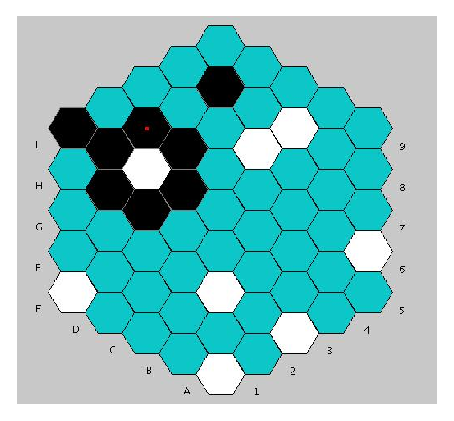
\epsfig{file=newFig1a.eps,width=30mm,height=30mm}\ 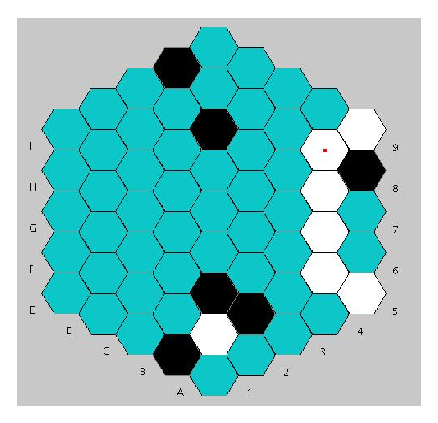
\epsfig{file=newFig1b.eps,width=30mm,height=30mm}\ 
\epsfig{file=newFig1c.eps,width=30mm,height=30mm}
\caption{\label{laFigQuiDitTout}Three finished games: a ring (a loop, by black), a bridge (linking two corners, by white), and a fork (linking three edges, by black).}
\end{figure}
\end{center}

The game of Havannah is particularly difficult for computers, for different reasons. We mention four of them.
\begin{itemize}
\item First, due to the large action space. For instance, in size 10 (10 locations per edge) there are 271 possible moves for the first player.
\item Second, there is no pruning rule for reducing the tree of the possible futures.
\item Third, there is no natural evaluation function.
\item Finally, the lack of expert knowledge for this game.
\end{itemize}
The efficiency of the MCTS algorithm on this game has been shown recently in \cite{fabienHavannah}. As far as we know, nowadays, all the robots which play this game use an MCTS algorithm. In their paper, they also have shown the efficiency of the RAVE formula.

%\subsubsection{Results}

%The experimental results are presented in Table \ref{hav1000}.

\begin{table}
\begin{tabular}{|c|c|c|c|}
\hline
 \# of simulations & Value of $p$ & Size of the pool & Success rate against the baseline \\
\hline
%$\frac{1}{2}$ & 10 & 54.32$\pm$0.46\% \\
%$          1$ & 10 & 52.42$\pm$0.70\% \\
%$\frac{1}{4}$ & 10 & 53.19$\pm$0.68\% \\
%$\frac{3}{4}$ & 10 & 53.34$\pm$0.85\% \\

1000 & $1/2$ & 5 & 52.70$\pm$0.62\% \\
1000 & $1/2$ & 10 & 54.32$\pm$0.46\% \\
1000 & $          1$ & 10 & 52.42$\pm$0.70\% \\
1000 & $1/4$ & 10 & 53.19$\pm$0.68\% \\
1000 & $3/4$ & 10 & 53.34$\pm$0.85\% \\
1000 & $          1$ & 20 & 53.20$\pm$0.80\% \\
1000 & $1/2$ & 20 & 52.51$\pm$0.54\% \\
1000 & $1/4$ & 20 & 52.13$\pm$0.55\% \\
1000 & $3/4$ & 20 & 52.90$\pm$0.34\% \\
10,000 & $1/2$ & 10 & 54.45$\pm$0.75\% \\
20,000 & $1/2$ & 10 & 54.42$\pm$0.89\% \\


\hline
\end{tabular}
\caption{\label{hav1000}Success rate of the poolRave modification for the game of Havannah. The baseline is the code without the poolRave modification.}
\end{table}


To improve the results by \cite{fabienHavannah} we applied the modification presented in section 3 for the game of Havannah. We measured the success rate of our bot with the new modification against the baseline version of our bot. There are two different parameters to tune : (i) $p$ which is the probability of playing a modified move and (ii) the size of the pool.
We have experimented with different numbers of simulations in order to see the robustness of our modification.
Results are shown in Table \ref{hav1000}. The best results are obtained with $p=1/2$ and a pool size of 10, for which we have a success rate of $54.32\%$ for 1,000 simulations and $54.45\%$ for 10,000 simulations. With the same set of parameters, for 20,000 simulations we have $54.42\%$. So, for the game of Havannah this improvement seems to be independent of the number of simulations.



\subsection{Go}\label{go}

 The game of Go is a classical benchmark for MCTS; this Asian game is probably the main challenge in games and a major testbed for artificial intelligence. The rules can be found on \url{http://senseis.xmp.net}; roughly, each player puts a stone of his color in turn, groups are maximum sets of connected stones for 4-connectivity, groups that do not touch any empty location are ``surrounded'' and removed from the board; the player who surround the bigger space with his\footnote{For brevity we use 'he' and 'his' whenever 'he or she' and 'his or her'are meant.} stones has won. Computers are far from the level of professional players in Go, and the best MCTS implementations for the game of Go use sophisticated Monte-Carlo Tree Search.

The modification proposed in this article is implemented in the Go program MoGo. The probability of using the modification $p$ is useful in order to preserve the diversity of the simulations. As, in MoGo, this role is already played by the ``fillboard'' modification \cite{peacg}, the probability $p$ is set to $1$. 
The experiments are done by making the original version of MoGo play against the version with the modification on a $9$x$9$ board with $1000$ simulations per move.

We obtain up to $51.7\pm0.5\%$ of victory. The improvement is mathematically significant but not very important. The reason is that Monte Carlo simulations in the program MoGo possess extensive domain knowledge in the form of patterns. In order to measure the effect of our modification in applications where no knowledge is available, we run more experiments with a version of MoGo without patterns. The results are presented in Table \ref{go1000}.


%%\subsubsection{Rules}

%%\subsubsection{Results}
\begin{table}
\begin{center}
\begin{tabular}{|c|c|c|c|}
\hline
 Size of the pool & Success rate against the baseline \\
\hline
5 & 54.2$\pm$1.7\% \\ 
10 & 58.7$\pm$0.6\% \\
20 & 62.7$\pm$0.9\% \\
30 & 62.7$\pm$1.4\% \\
60 & 59.1$\pm$1.8\% \\
%$          1$ & 100 & inf 50 & 58.3$\pm$2.4\% \\
%$          1$ & 20 & inf 200 & 61.4$\pm$1.4\% \\
%$          1$ & 20 & inf 500 & 62.4$\pm$1.8\% \\
%$          1$ & 20 & inf 5000 & 60.9$\pm$1.2\% \\
%$          1$ & 20 & inf 0 & 56.9$\pm$1.7\% \\

\hline
\end{tabular}
\caption{\label{go1000}Success rate of the poolRave modification for the game of Go. The baseline is the code without the poolRave modification. This is in the case of no patterns in the Monte-Carlo part.}
\end{center}
\end{table}


%$          1$ & 20 & inf 50 & 51.7$\pm$0.5\% \\
%\caption{\label{hav1000}500 simulations with Pattern .}



When the size of the pool is too large or not large enough, the modification is not as efficient.
When using a good compromise for the size ($20$ in the case of MoGo for $9$x$9$ Go), we obtain $62.7\pm0.9\%$ of victory.

It is also interesting to note that when we increase the number of simulations per move, we obtain slightly better results. For example, with 10,000 simulations per move, we obtain $64.4\pm0.4\%$ of victory.



\section{Conclusion}

We presented a generic way of improving the Monte-Carlo simulations in the Monte-Carlo Tree Search algorithm called PoolRave (see section 3). This method is based on already existing values (the RAVE values) and is easy to implement.

We show two different applications where this improvement was successful: the game of Havannah and the game of Go. 
For the game of Havannah, we achieve $54.3\%$ of victory against the version without the modification.
For the game of Go, we achieve only $51.7\%$ of victory against the version without modification. However, without the domain-specific knowledge, we obtain up to $62.7\%$ of victory. So, we may conclude that the modification is worthwhile to implement.

In the near future, we intend to use an evolution algorithm in order to tune the different parameters. We will also try different ways of using these values in order to improve the Monte-Carlo simulations. We strongly believe that the next step in improving the MCTS algorithm will be reached by finding an efficient way of modifying the Monte-Carlo simulations depending on the context.



\bibliographystyle{abbrv}
\bibliography{tout}

\end{document}
